%%%%%%%%%%%%%%%%%%%%%%%%%%%%%%%%%%%%%%%%%%%%%%%%%%%%%%%%%%%%%%%%%%
%  = PREAMBLE =
% The preamble of a LaTeX document is the set of commands that 
%    precede the \begin{document} line.  It sets up the style of 
%    the document.
%%%%%%%%%%%%%%%%%%%%%%%%%%%%%%%%%%%%%%%%%%%%%%%%%%%%%%%%%%%%%%%%%%

\documentclass[aps,twocolumn, secnumarabic,balancelastpage,amsmath,amssymb,nofootinbib,floatfix]{revtex4-1}

\usepackage{graphicx}      % tools for importing graphics
\usepackage{tikz}
\usepackage{tikz-feynman}  % Requires TikZ-Feynman package
\usepackage{parskip}
\usepackage[colorlinks=true]{hyperref}  % this package should be added after 
                                        % all others.
                                        % usage: \url{http://web.mit.edu/8.13}

\setlength{\parskip}{5pt}
\usetikzlibrary{decorations.pathmorphing}

%%%%%%%%%%%%%%%%%%%%%%%%%%%%%%%%%%%%%%%%%%%%%%%%%%%%%%%%%%%%%%%%%%%
% And now, begin the document...
%%%%%%%%%%%%%%%%%%%%%%%%%%%%%%%%%%%%%%%%%%%%%%%%%%%%%%%%%%%%%%%%%%%

\begin{document}

\title{Random Number Generator from Atomospheric Muon Detection}% \author{Vinh Tran}
% \email{vinhtran@mit.edu}
\author{Yongao Hu}
\email{yongao@mit.edu}
\date{\today}
\affiliation{MIT Department of Physics}


\begin{abstract}
This report presents a statistical analysis on the random nature of atmospheric muon detection. The analysis is based on the data collected by the Cosmic Muon Detector at MIT, which detects atmospheric muons produced by cosmic rays interacting with the Earth's atmosphere. The data is analyzed using statistical methods to determine the random nature of the muon detection process. The analysis includes the monobit frequency test, sequence test, autocorrelation function, compression ratio, Shannon entropy, Lempel-Ziv complexity, and dependence on angle of the detectors. The results show that the muon detection process is indeed random, and independent of the angle of the detectors. The results are consistent with the expected behavior of a random process, with deviation of $0.40\sigma$, showing that the muon detection process can be used as a source of true random numbers. 
\end{abstract}

\maketitle

\section{Introduction}
Random number generators produces numbers that are uniformly distributed over a range of values. True random numbers are surprisingly difficult to generate because most conventional methods rely on deterministic algorithms, which can only produce pseudo-randomness rather than true unpredictability. Yet, many critical applications — from cryptography to scientific simulations — depend on genuinely random numbers to ensure security and accuracy. This scarcity of reliable, truly random sources has driven researchers to explore natural phenomena as entropy sources. Atmospheric muons, high-energy particles generated from cosmic rays interacting with Earth's atmosphere, arrive at random times and locations, making them an excellent candidate for a truly random number generator. We aim to test if the muon detection process is random and can be used as a source of true random numbers. 

Atomospheric muons are produced by cosmic rays interacting with the Earth's atmosphere. Primary cosmic rays, typically protons or heavier nuclei, collide with atmospheric nuclei at altitudes of 15--20 km, producing showers of secondary particles. Most of the collision energy goes into creating mesons, primarily pions and kaons. Charged mesons decay into muons and neutrinos, while neutral mesons rapidly decay into gamma rays. The cosmic-ray muons observed at ground level predominantly originate from the decay of charged pions, and to a lesser extent from kaon decays. Although the primary cosmic rays are absorbed high in the atmosphere, secondary muons, due to their relatively long lifetime and high energy, can penetrate to the Earth's surface \cite{axani2024cosmicwatch}.

\section{Experimental Setup}
The Cosmic Muon Detector at MIT consists of a scintillator that emits light when a muon passes through it, and a photomultiplier tube (PMT) that detects the light and produces an electrical signal. The PMT signal is then processed to determine the time and energy of the muon detection event \cite{axani2024cosmicwatch}. We only count the event if two detectors placed 5 cm apart are triggered at the same time. The coincidence events indicate that the muon passed through both detectors. 

We also take data at different incident angle of the detectors to see if the angle has any effect on the random nature of the data. The detectors are secured at a fixed angle, varied from 0 to 90 degrees in increments of 10 degrees. The data is collected for each angle for a period of time ranging from 24 to 96 hours. 

The number and timestamps of muon detection events is recorded. The data is then analyzed using statistical methods to determine the random nature of the muon detection process.

\section{Data Analysis}

\subsection{Monobit Frequency Test}
In order to analyze the random nature of the data, we take the timestamp of the events and convert them to 0 if the timestamp is even and 1 if the timestamp is odd \cite{axani2024cosmicwatch}. This gives us a binary sequence of 0s and 1s. We then calculate the probability of getting a 1 in the sequence, which should be close to 0.5 if the data is random. We also choose the data with voltage higher than 80 mV to ensure that the data is not affected by gamma rays \cite{axani2024cosmicwatch}. 

We also calculate the cumulative frequency of the binary sequence. The cumulative frequency is defined as:
\begin{equation}
F(x) = \frac{1}{N} \sum_{i=0}^{N-1} x_i
\end{equation}
where $N$ is the total number of events, $x_i$ is the binary sequence, and $F(x)$ is the cumulative frequency. The cumulative frequency should be close to 0.5 if the data is random.

\subsection{Sequence Test}
We also conduct a sequence test to check for the presence of long-range correlations in the data. We convert the consecutive events into an $n$-bit binary sequence, where $n$ is the number of bits to make up each number. We then plot the probability of each bit against the possible number that can be generated. The plot should show a uniform distribution if the data is random. 

\subsection{Autocorrelation Function}
In order to further test the long-range correlation of the data, we calculate the autocorrelation function of the binary sequence. The autocorrelation function is defined as \cite{brockwell1991timeseries}:
\begin{equation}
R(\tau) = \frac{1}{N} \sum_{i=0}^{N-\tau-1} (x_i - \bar{x})(x_{i+\tau} - \bar{x})
\end{equation}
where $N$ is the total number of events, $x_i$ is the binary sequence, $\bar{x}$ is the mean of the binary sequence, and $\tau$ is the time lag. 

If there is no correlation, the expected value of the autocorrelation function is approximated to be
\begin{equation}
R(\tau) \approx \sigma \sqrt{\frac{2}{\pi}}
\end{equation}
where $\sigma$ is the standard deviation of the binary sequence. 

\subsection{Compression Ratio}
We also calculate the compression ratio of the binary sequence with compression algorithm \textsc{gzip} \cite{gzip}. The compression ratio is defined as:
\begin{equation}
\operatorname{CR} = \frac{L_{\text{original}}}{L_{\text{compressed}}}
\end{equation}
where $L_\text{original}$ is the length of the original binary sequence and $L_\text{compressed}$ is the length of the compressed binary sequence. The compression ratio should be close to 1 if the data is random. This is because a random sequence does not have any long-range correlations, and thus the compression algorithm cannot compress the data. 

\subsection{Entropy}
We also calculate the entropy of the binary sequence using the Shannon entropy formula \cite{shannon1948mathematical}:
\begin{equation}
H(X) = -\sum_{i=0}^{n-1} p(x_i) \log_2 p(x_i)
\end{equation}
where $p(x_i)$ is the probability of getting a 1 in the sequence at position $i$. The entropy should be close to 1 if the data is random. 

\subsection{Lempel-Ziv Complexity}
The Lempel-Ziv complexity of a finite sequence $S = s_1 s_2 \dots s_n$ is defined as the number of distinct phrases one obtains when parsing $S$ sequentially \cite{lempel1976complexity}. We build a growing dictionary of substrings by scanning $S$ from left to right: at each step, the longest prefix of the remaining suffix that already appears in the dictionary is identified, and the next new symbol is appended to form a new dictionary entry.  The complexity $c(S)$ is then the total count of such dictionary entries at the end of the parse.  $c(S)$ measures the algorithmic novelty or unpredictability of $S$: highly regular or repetitive sequences admit few new phrases and thus have low complexity, whereas random or highly structured sequences generate many new phrases and yield high complexity. 

Let $S$ be a sequence of length $n$ drawn uniformly from $\{0,1\}$.  In this case, the Lempel-Ziv complexity $c(S)$ grows almost surely as
\begin{equation}
    c(S)\;\sim\;\frac{n}{\log_{2}n}\to n \text{ as } n\to\infty
\end{equation}

A random sequence yields nearly the maximal number of new phrases at each parsing step, so its complexity increases at the rate $n \log{n}$, sub-linear in $n$ but diverging without bound. 

\subsection{Angular Dependence Test}
To model the angular depedence on the random nature of the data, we take data at different angles and repeat the same analysis. We then fit the probability of getting a 1 in the sequence to a linear function of the angle. The gradient of the linear function should be close to 0 if the data is random.

\subsection{Uncertainty Analysis}
The primary source of uncertainty in our tests is the finite-sample fluctuations inherent to a stochastic muon-detection process.  We quantify the uncertainty of each statistic as follows:

\subsubsection{Uncertainty in the sample proportion}
Let $\hat p = \tfrac{1}{N}\sum_{i=1}^N x_i$ be the empirical probability of a “1” in the binary sequence of length $N$.  By the properties of a binomial distribution, the standard error of $\hat{p}$ is
\begin{equation}
\sigma_{\hat p}
= \sqrt{\frac{\hat p\,(1-\hat p)}{N}}
\end{equation}


\subsubsection{Uncertainty in the autocorrelation function}
For lag \(\tau\), the autocorrelation estimator has standard error approximately
\begin{equation}
\sigma_{R}(\tau) \approx \frac{1}{\sqrt{N-\tau}}
\end{equation}
assuming weak dependence at large $\tau$.

\subsubsection{Uncertainty in the compression ratio, Shannon entropy, and Lempel-Ziv complexity}
We estimate the error by \textit{nonparametric bootstrap}: we resample the binary sequence (with replacement) $B$ times, compute the statistic of interest for each resample, and report the mean and standard deviation of the resulting $B$ values. We take $B=10000$ in our analysis.

\subsubsection{sigificance of the results}
The significance of the results is calculated using the z-score, which is defined as:
\begin{equation}
z = \frac{x - \mu}{\sigma}
\end{equation}
where $x$ is the observed value, $\mu$ is the expected value, and $\sigma$ is the standard deviation. The significance level is set at 5\%, which corresponds to a z-score of 1.96. If the z-score is greater than 1.96, we reject the null hypothesis that the data is random. 

\section{Results}
\subsection{Monobit Frequency Test}
Firstly, we plot the count of 1 and 0 in the binary sequence in Fig. \ref{fig:monobit_histogram} and Fig. \ref{fig:running_frequency}. The total count of the bits is 1636. The monobit probability is $0.508 \pm 0.012$. The sigificance of the result compared to the expected value of 0.5 is $z=0.64$, which is not significant at the 5\% level. 
\begin{figure}
\centering
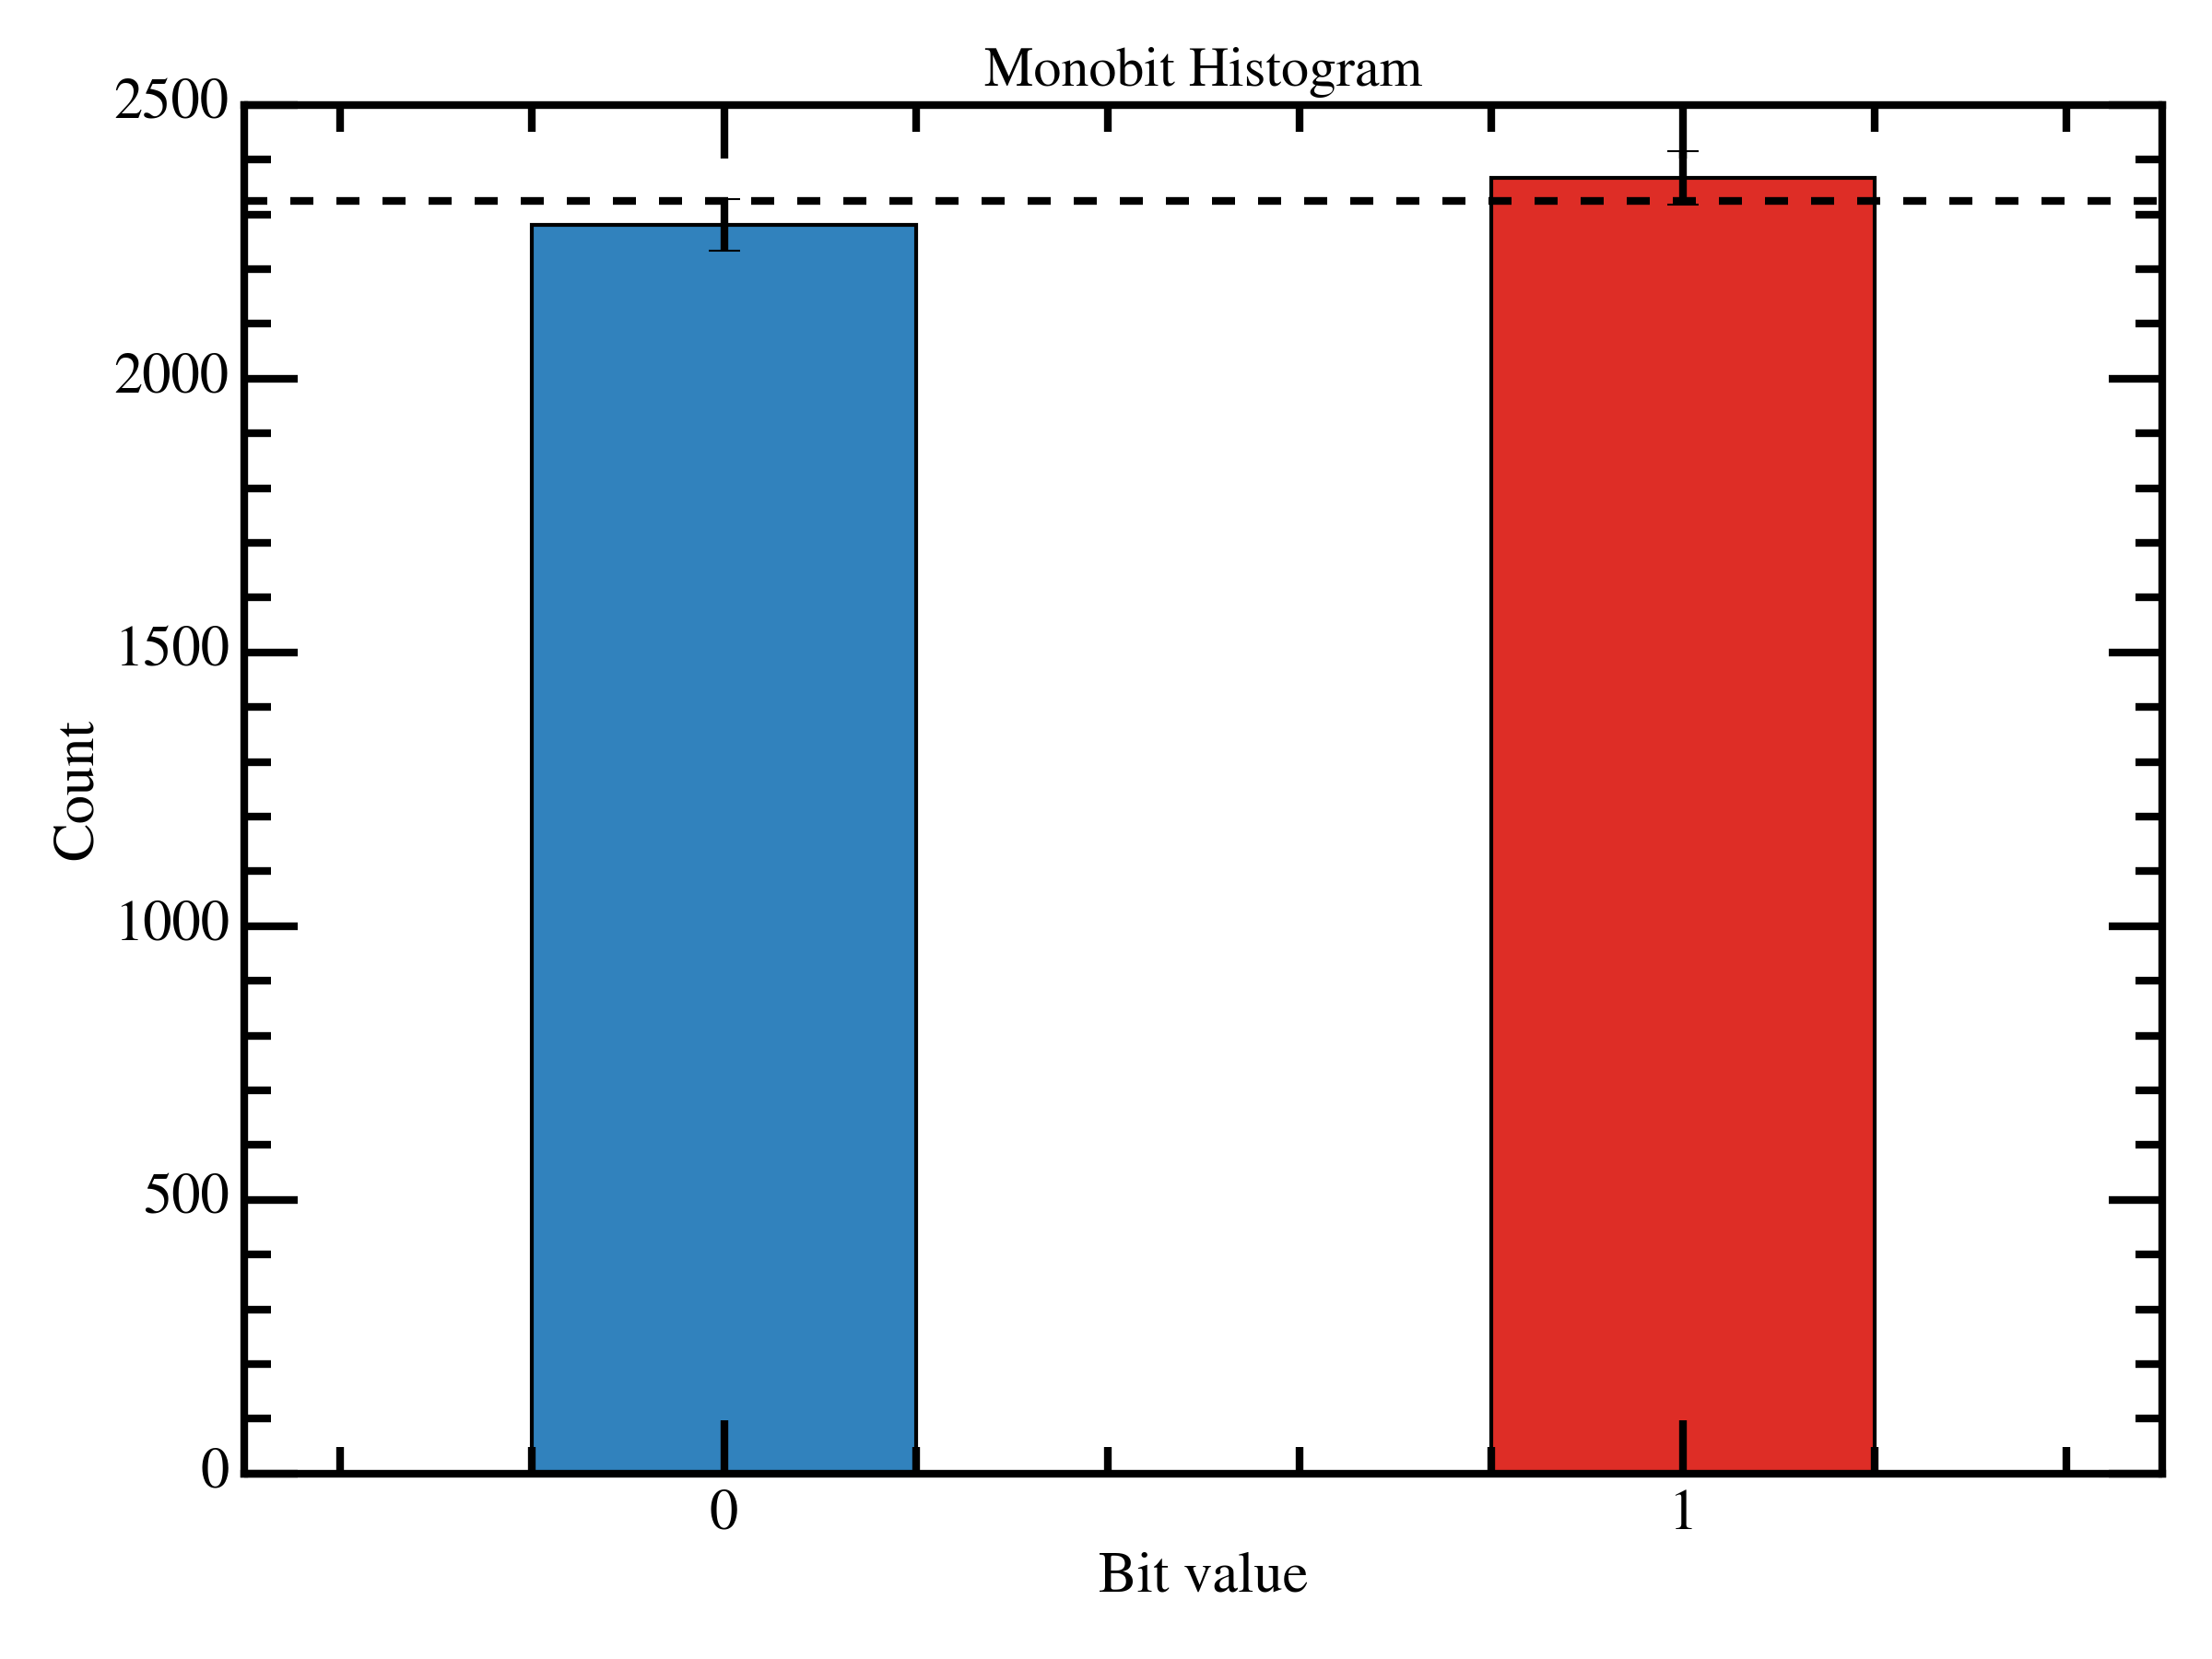
\includegraphics[width=0.45\textwidth]{figure/monobit_histogram.png}
\caption{Histogram of the binary sequence. The plot shows that the count of 1 and 0 is roughly equal, indicating that the data is random.}
\label{fig:monobit_histogram}
\end{figure}
\begin{figure}
\centering
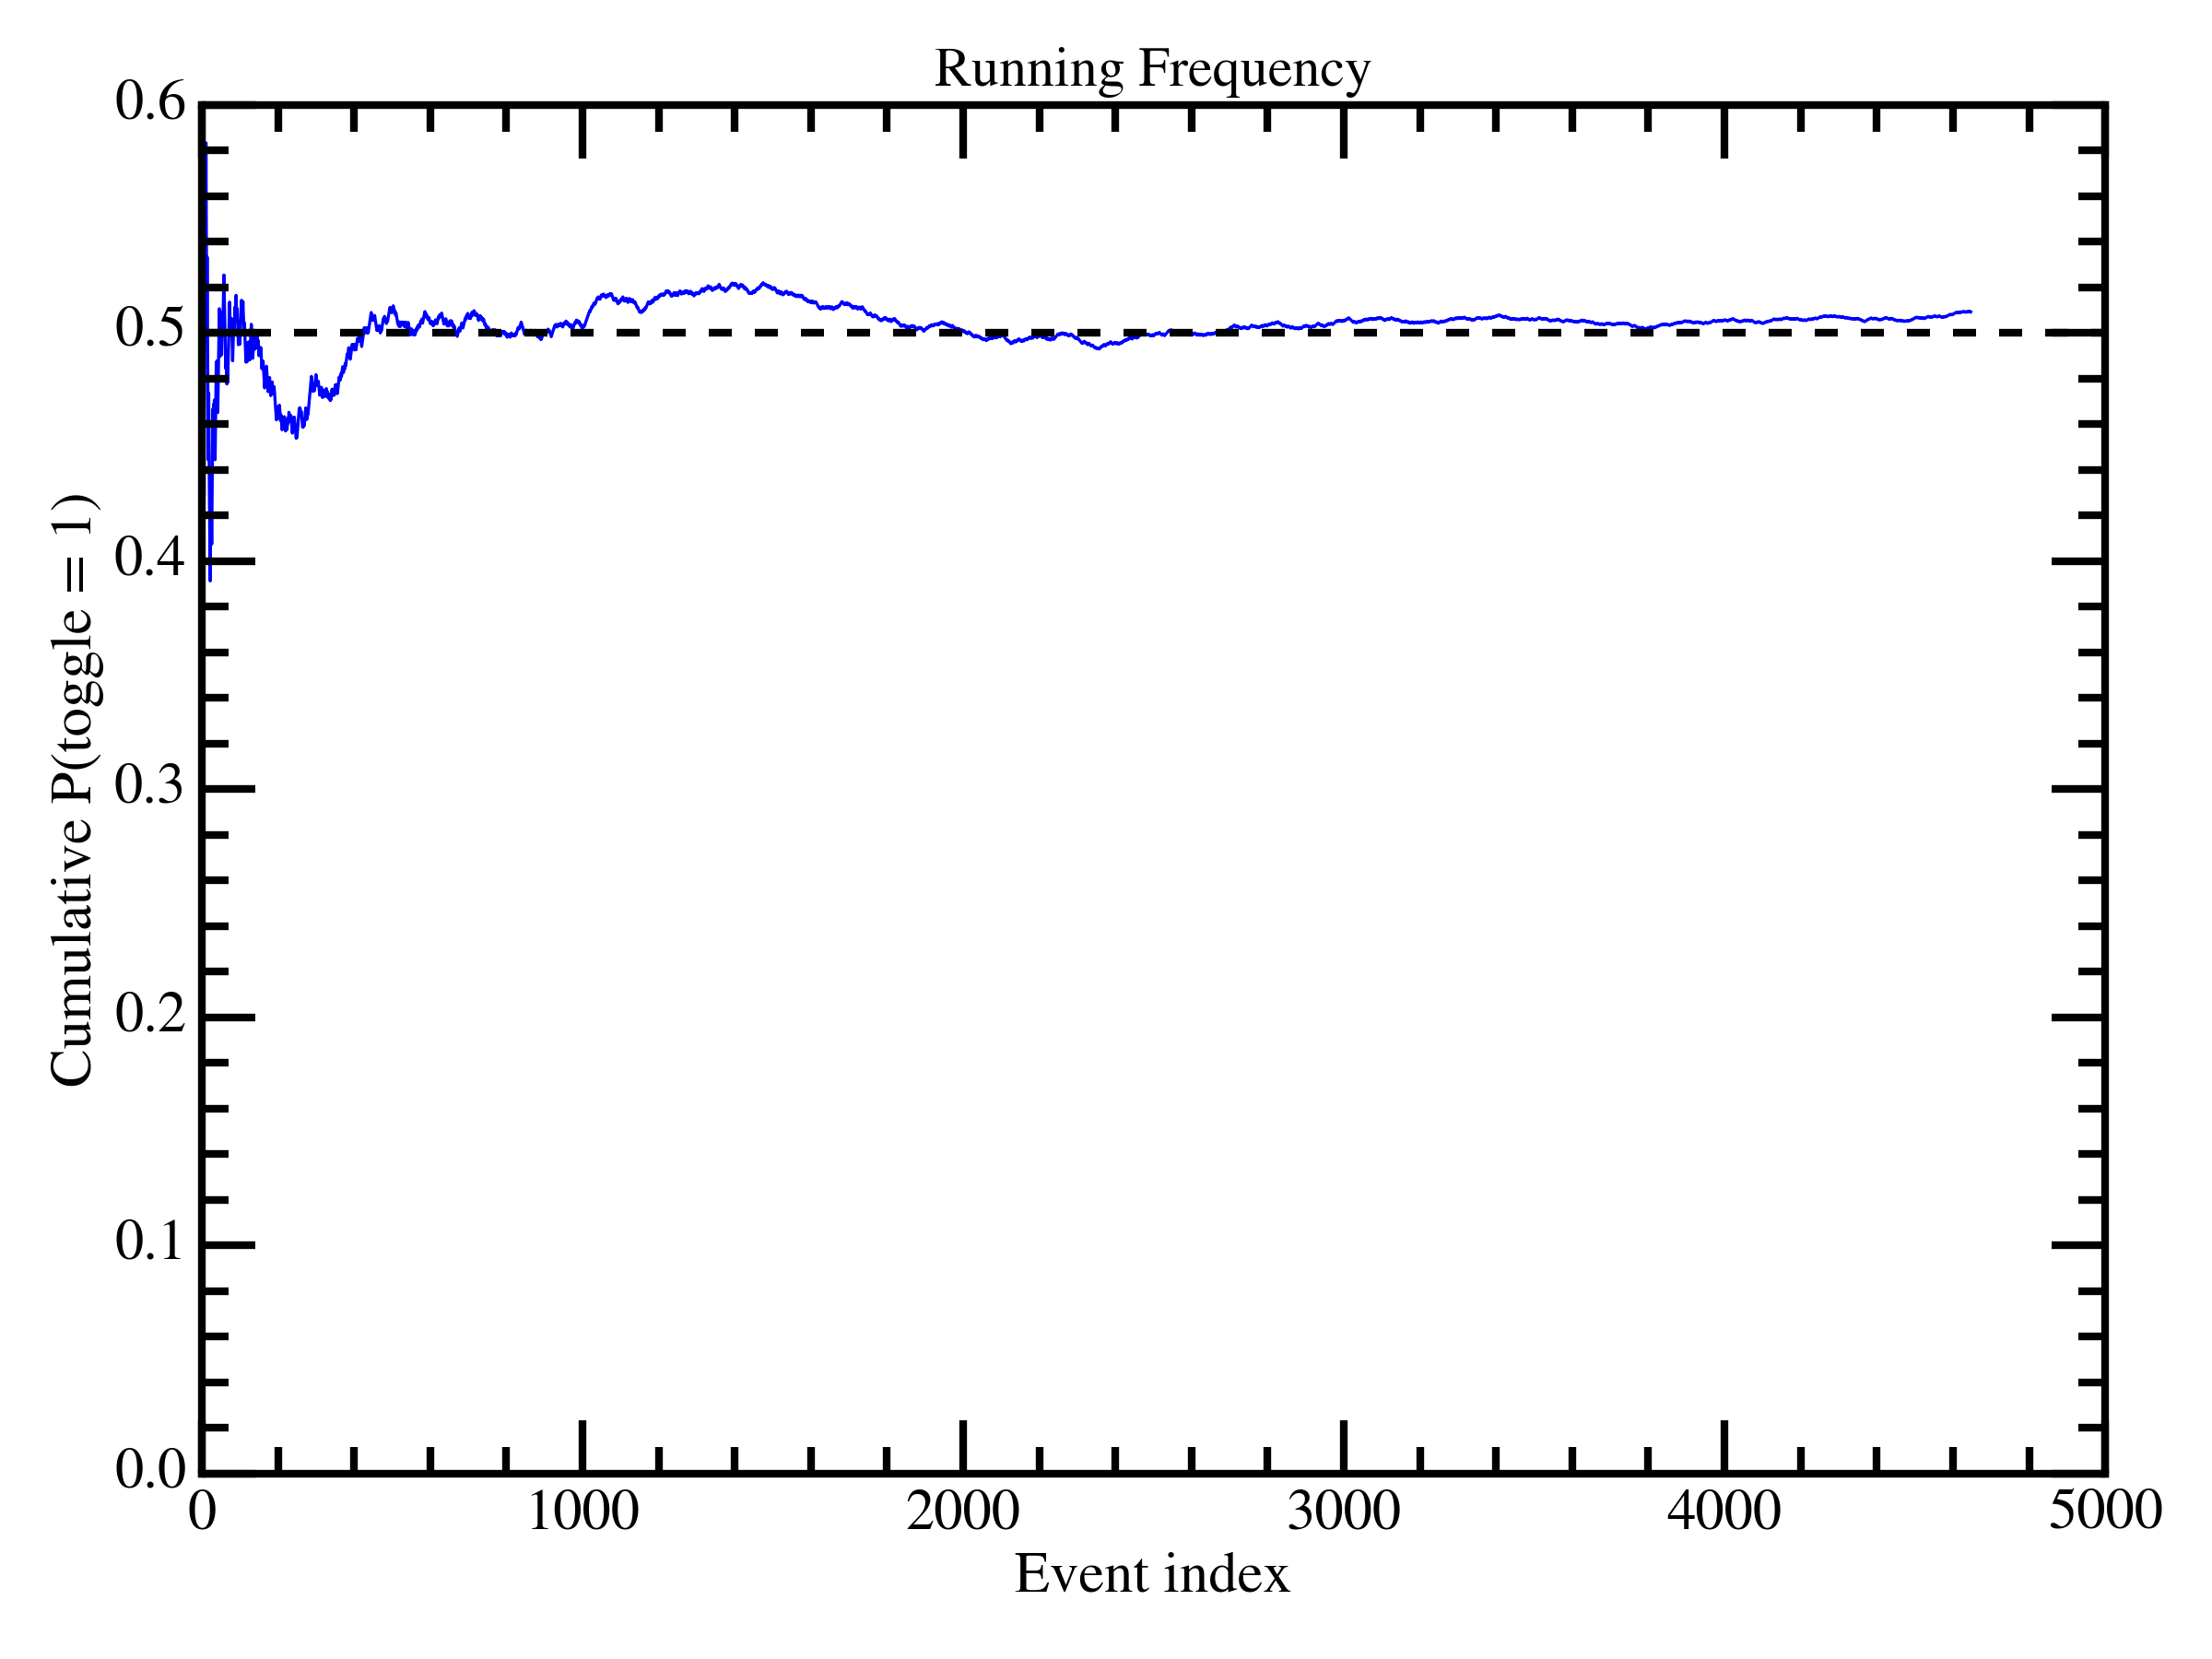
\includegraphics[width=0.45\textwidth]{figure/running_frequency.png}
\caption{Cumulative frequency of the binary sequence. The plot shows that the cumulative frequency of 1 and 0 is roughly equal, indicating that the data is random.}
\label{fig:running_frequency}

\end{figure}

\subsection{Sequence Test}

Next, we show the 4-bit and 6-bit binary sequence in Fig. \ref{fig:serial_4bit_6bit}. The plot shows that the probability of each bit is roughly equal, indicating that the data is random.
\begin{figure}
\centering
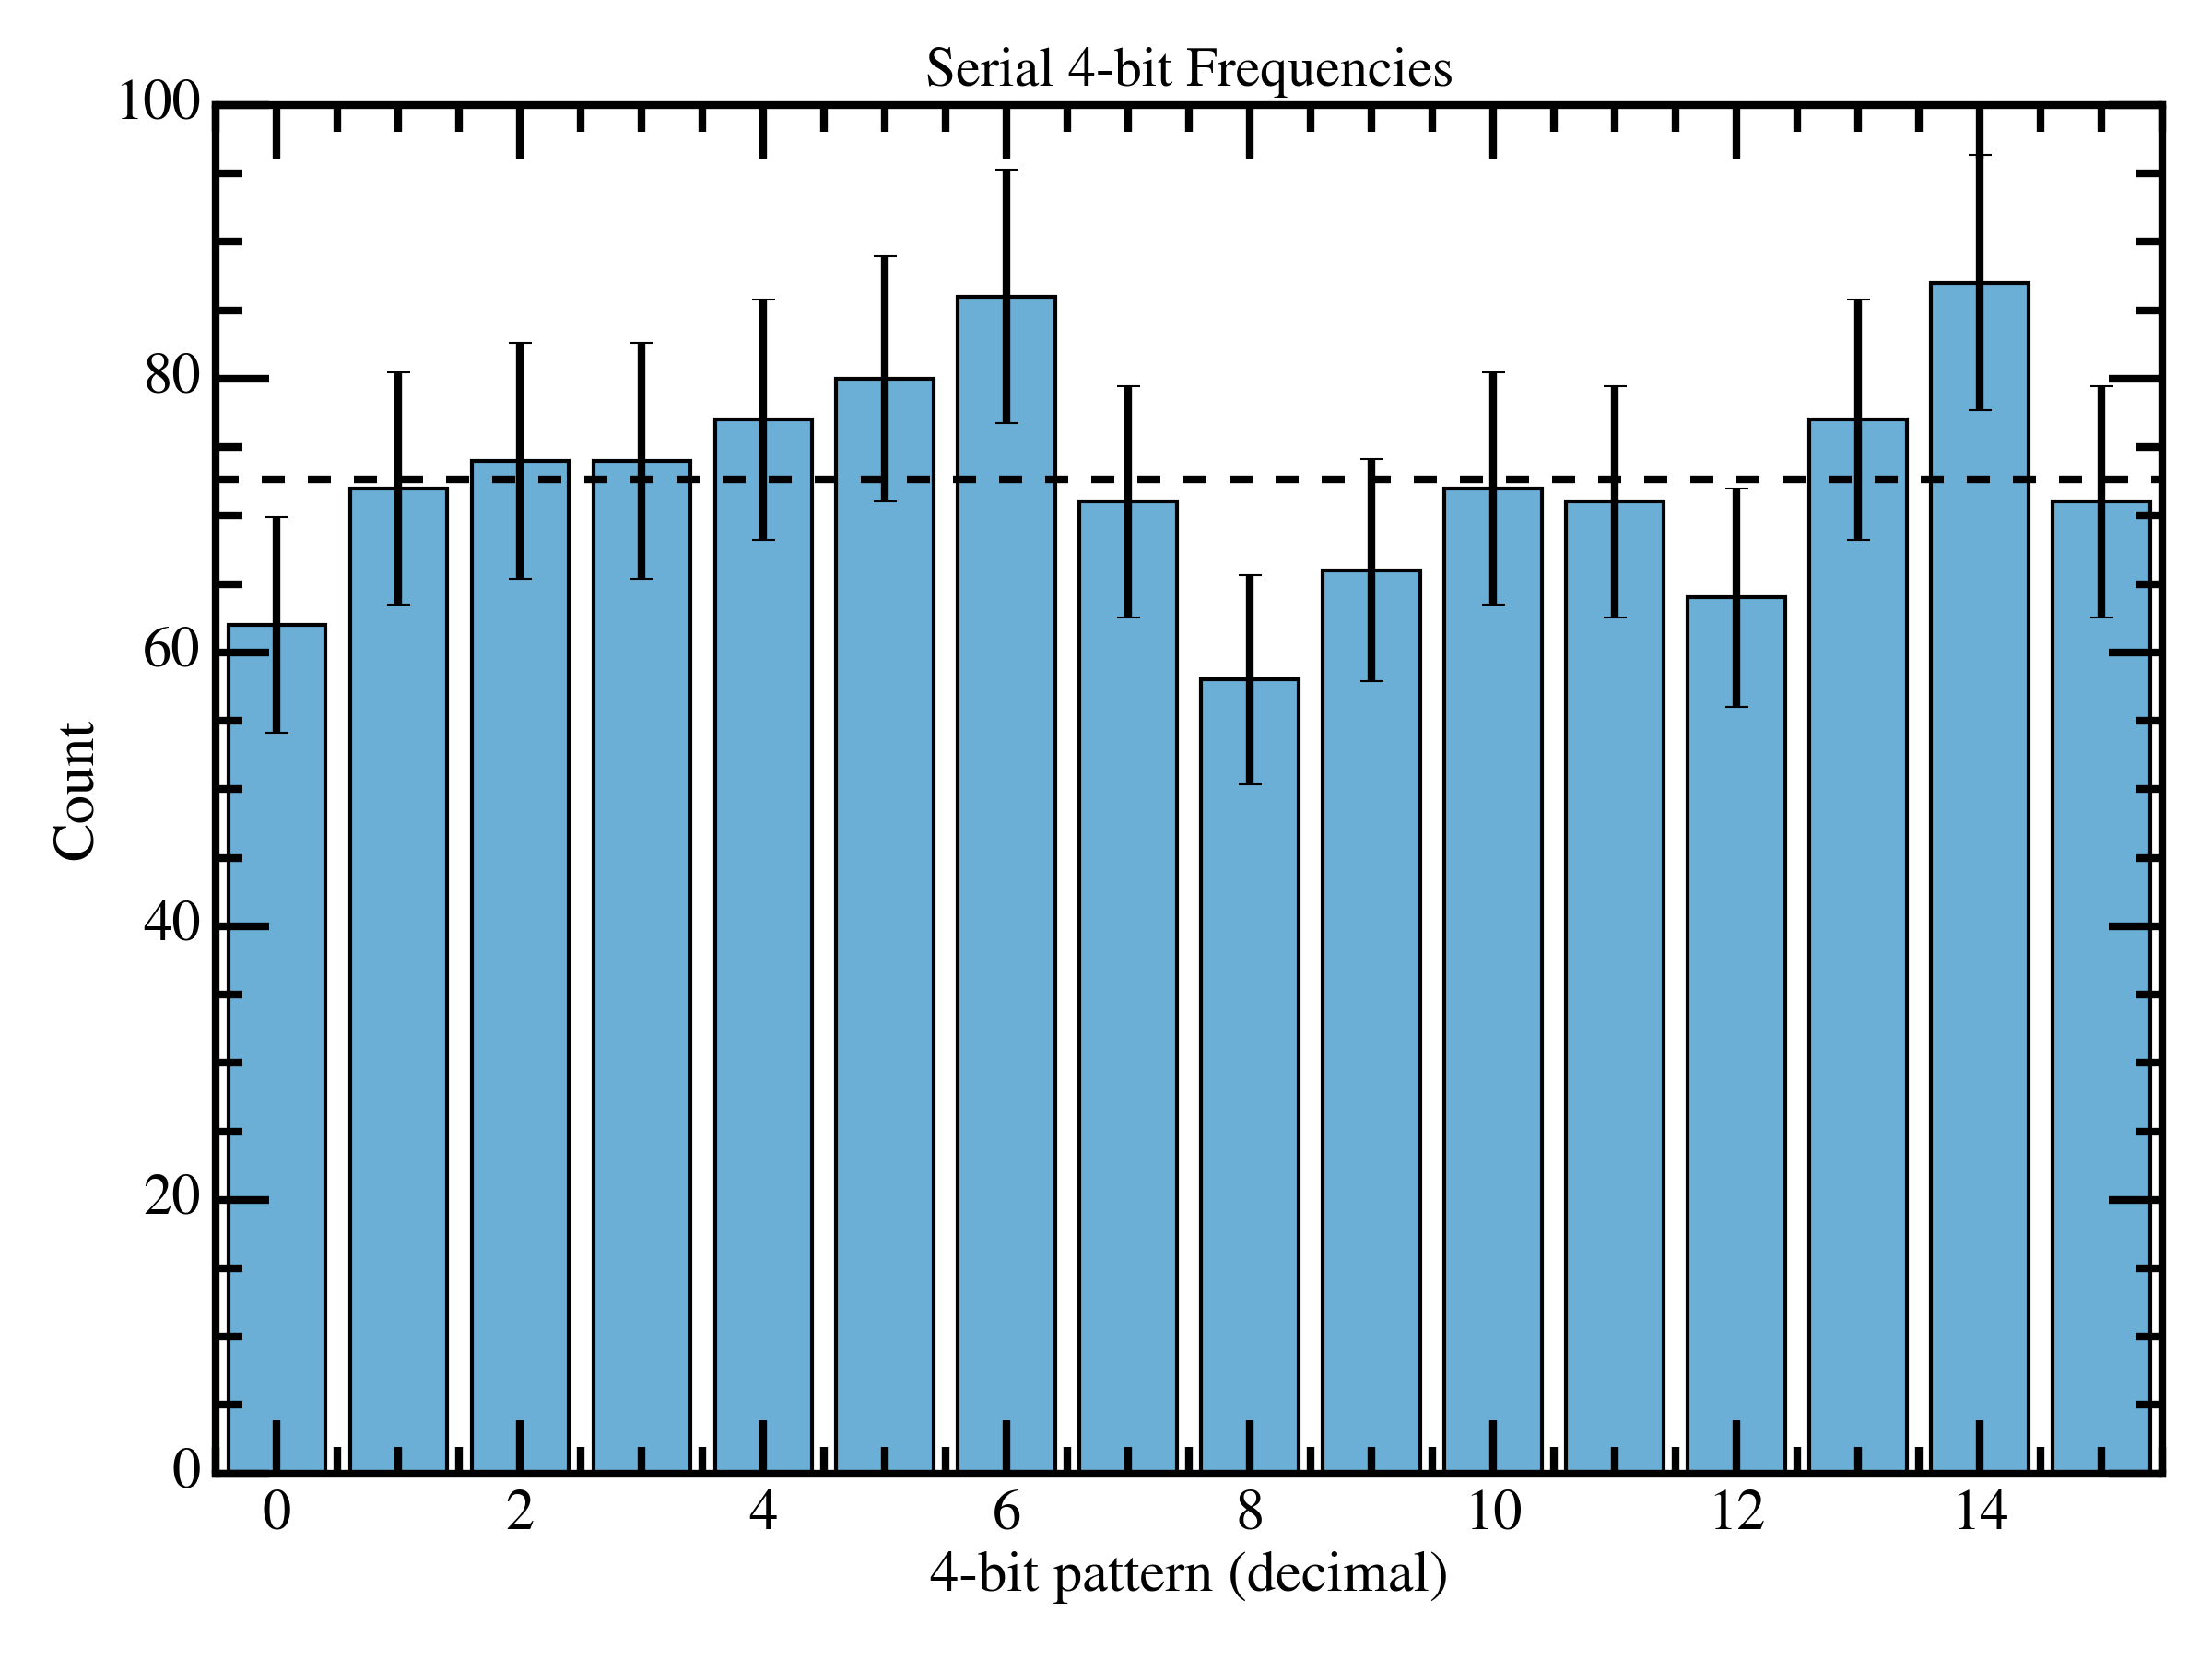
\includegraphics[width=0.45\textwidth]{figure/serial4.png}
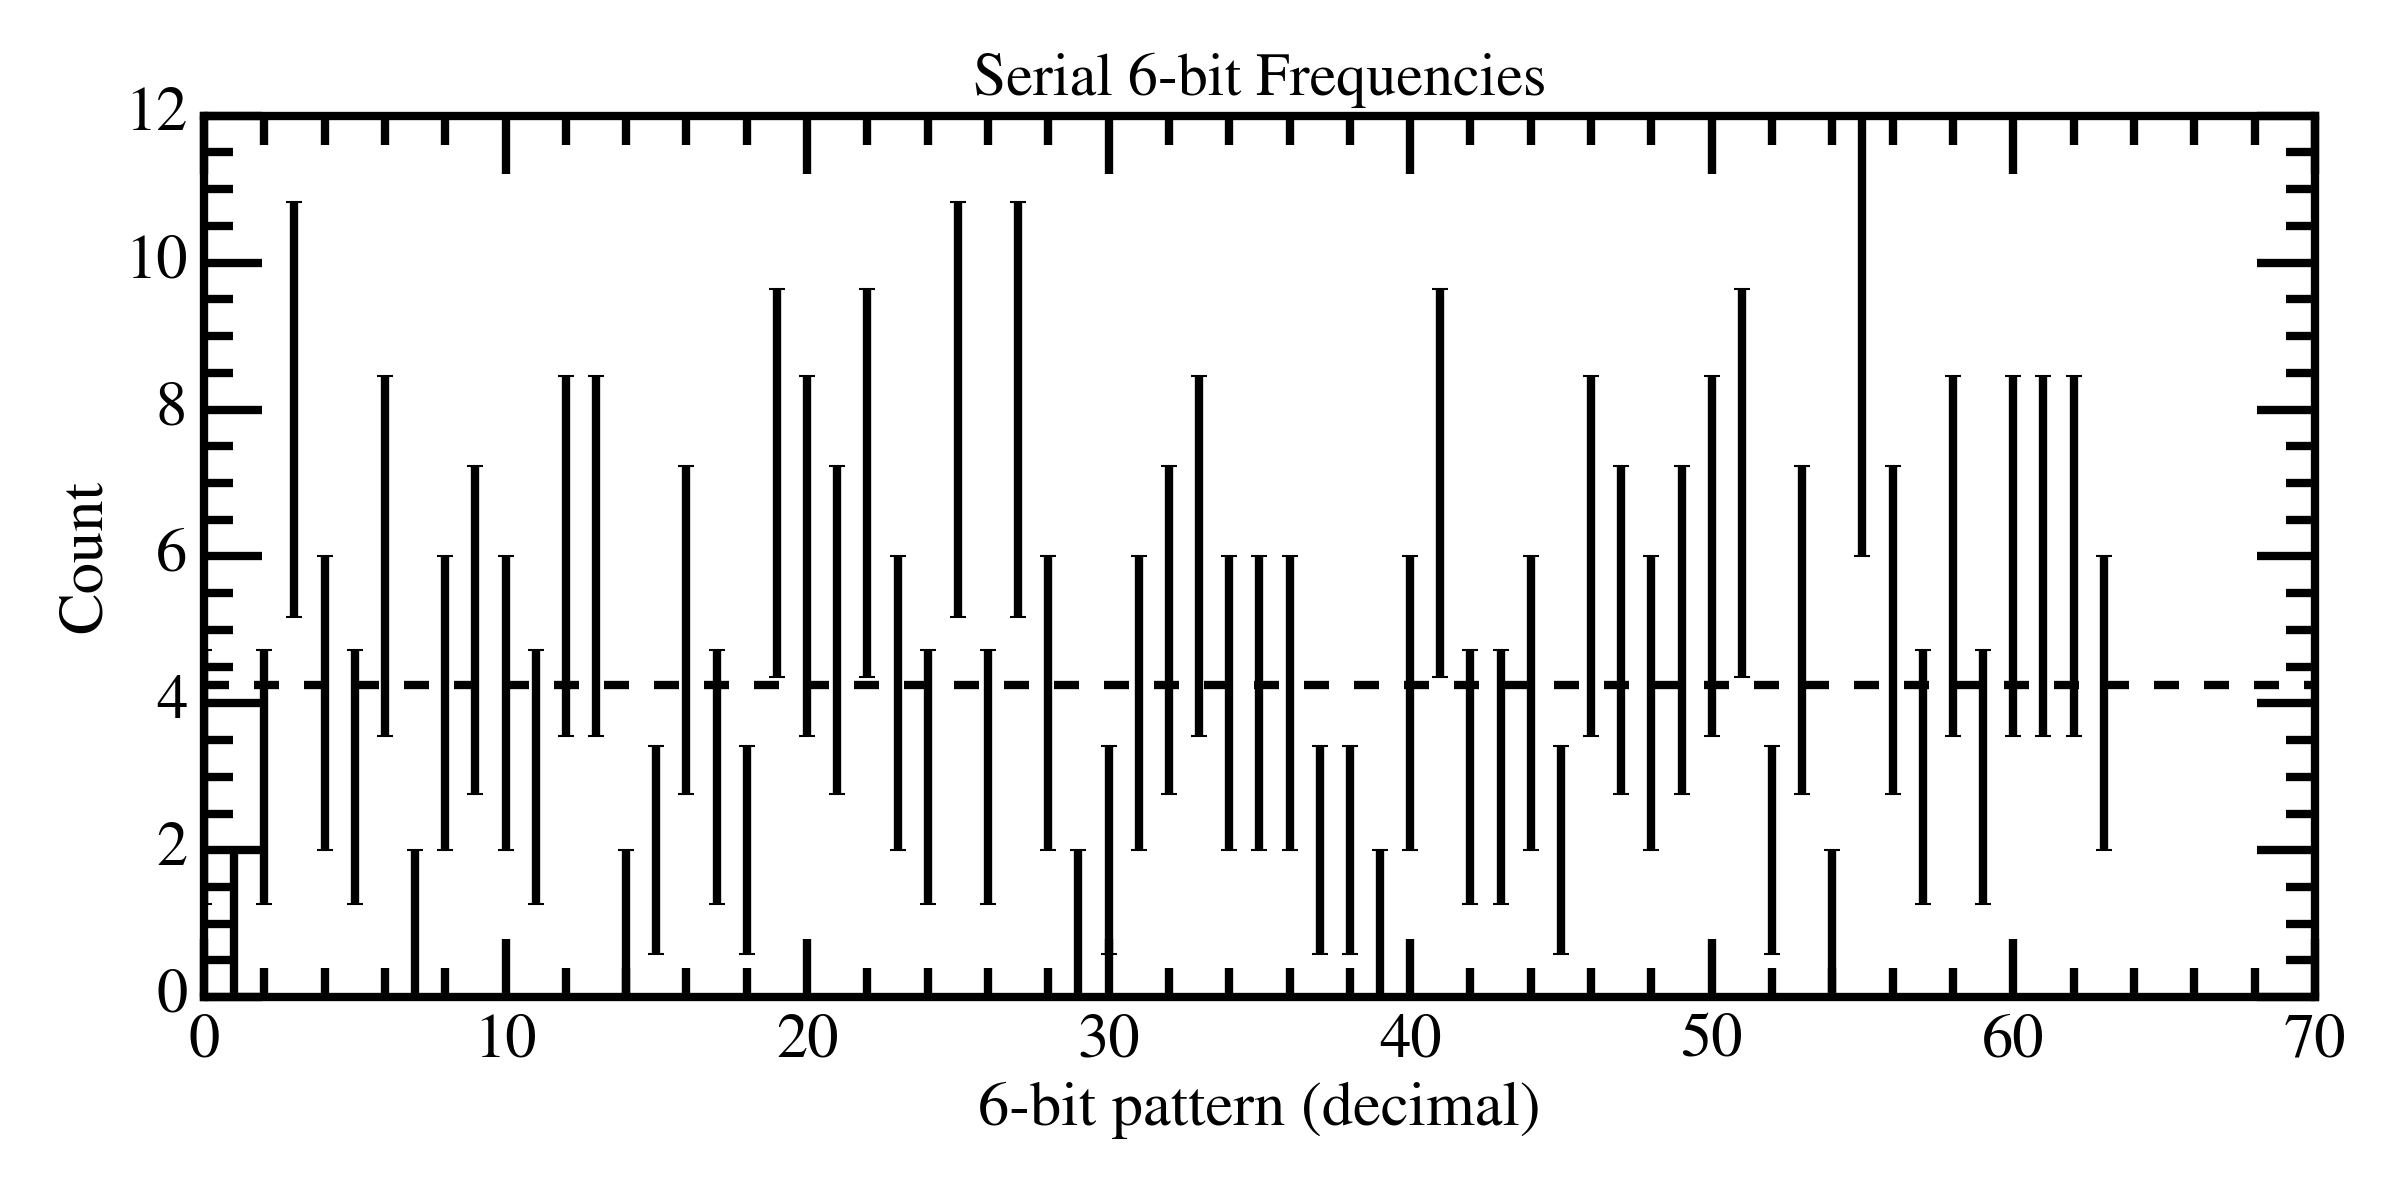
\includegraphics[width=0.45\textwidth]{figure/serial6.png}
\caption{4-bit and 6-bit binary sequence. The plot shows that the probability of each bit is roughly equal, indicating that the data is random.}
\label{fig:serial_4bit_6bit}
\end{figure}


\subsection{Autocorrelation Function}
Next, we show the autocorrelation function of the binary sequence in Fig. \ref{fig:autocorrelation}. The mean of the absolute value of the autocorrelation function is $0.0172 \pm 0.0024$. The significance of the result compared to the expected value of 0 is $z=1.06$, which is not significant at the 5\% level. 
\begin{figure}
\centering
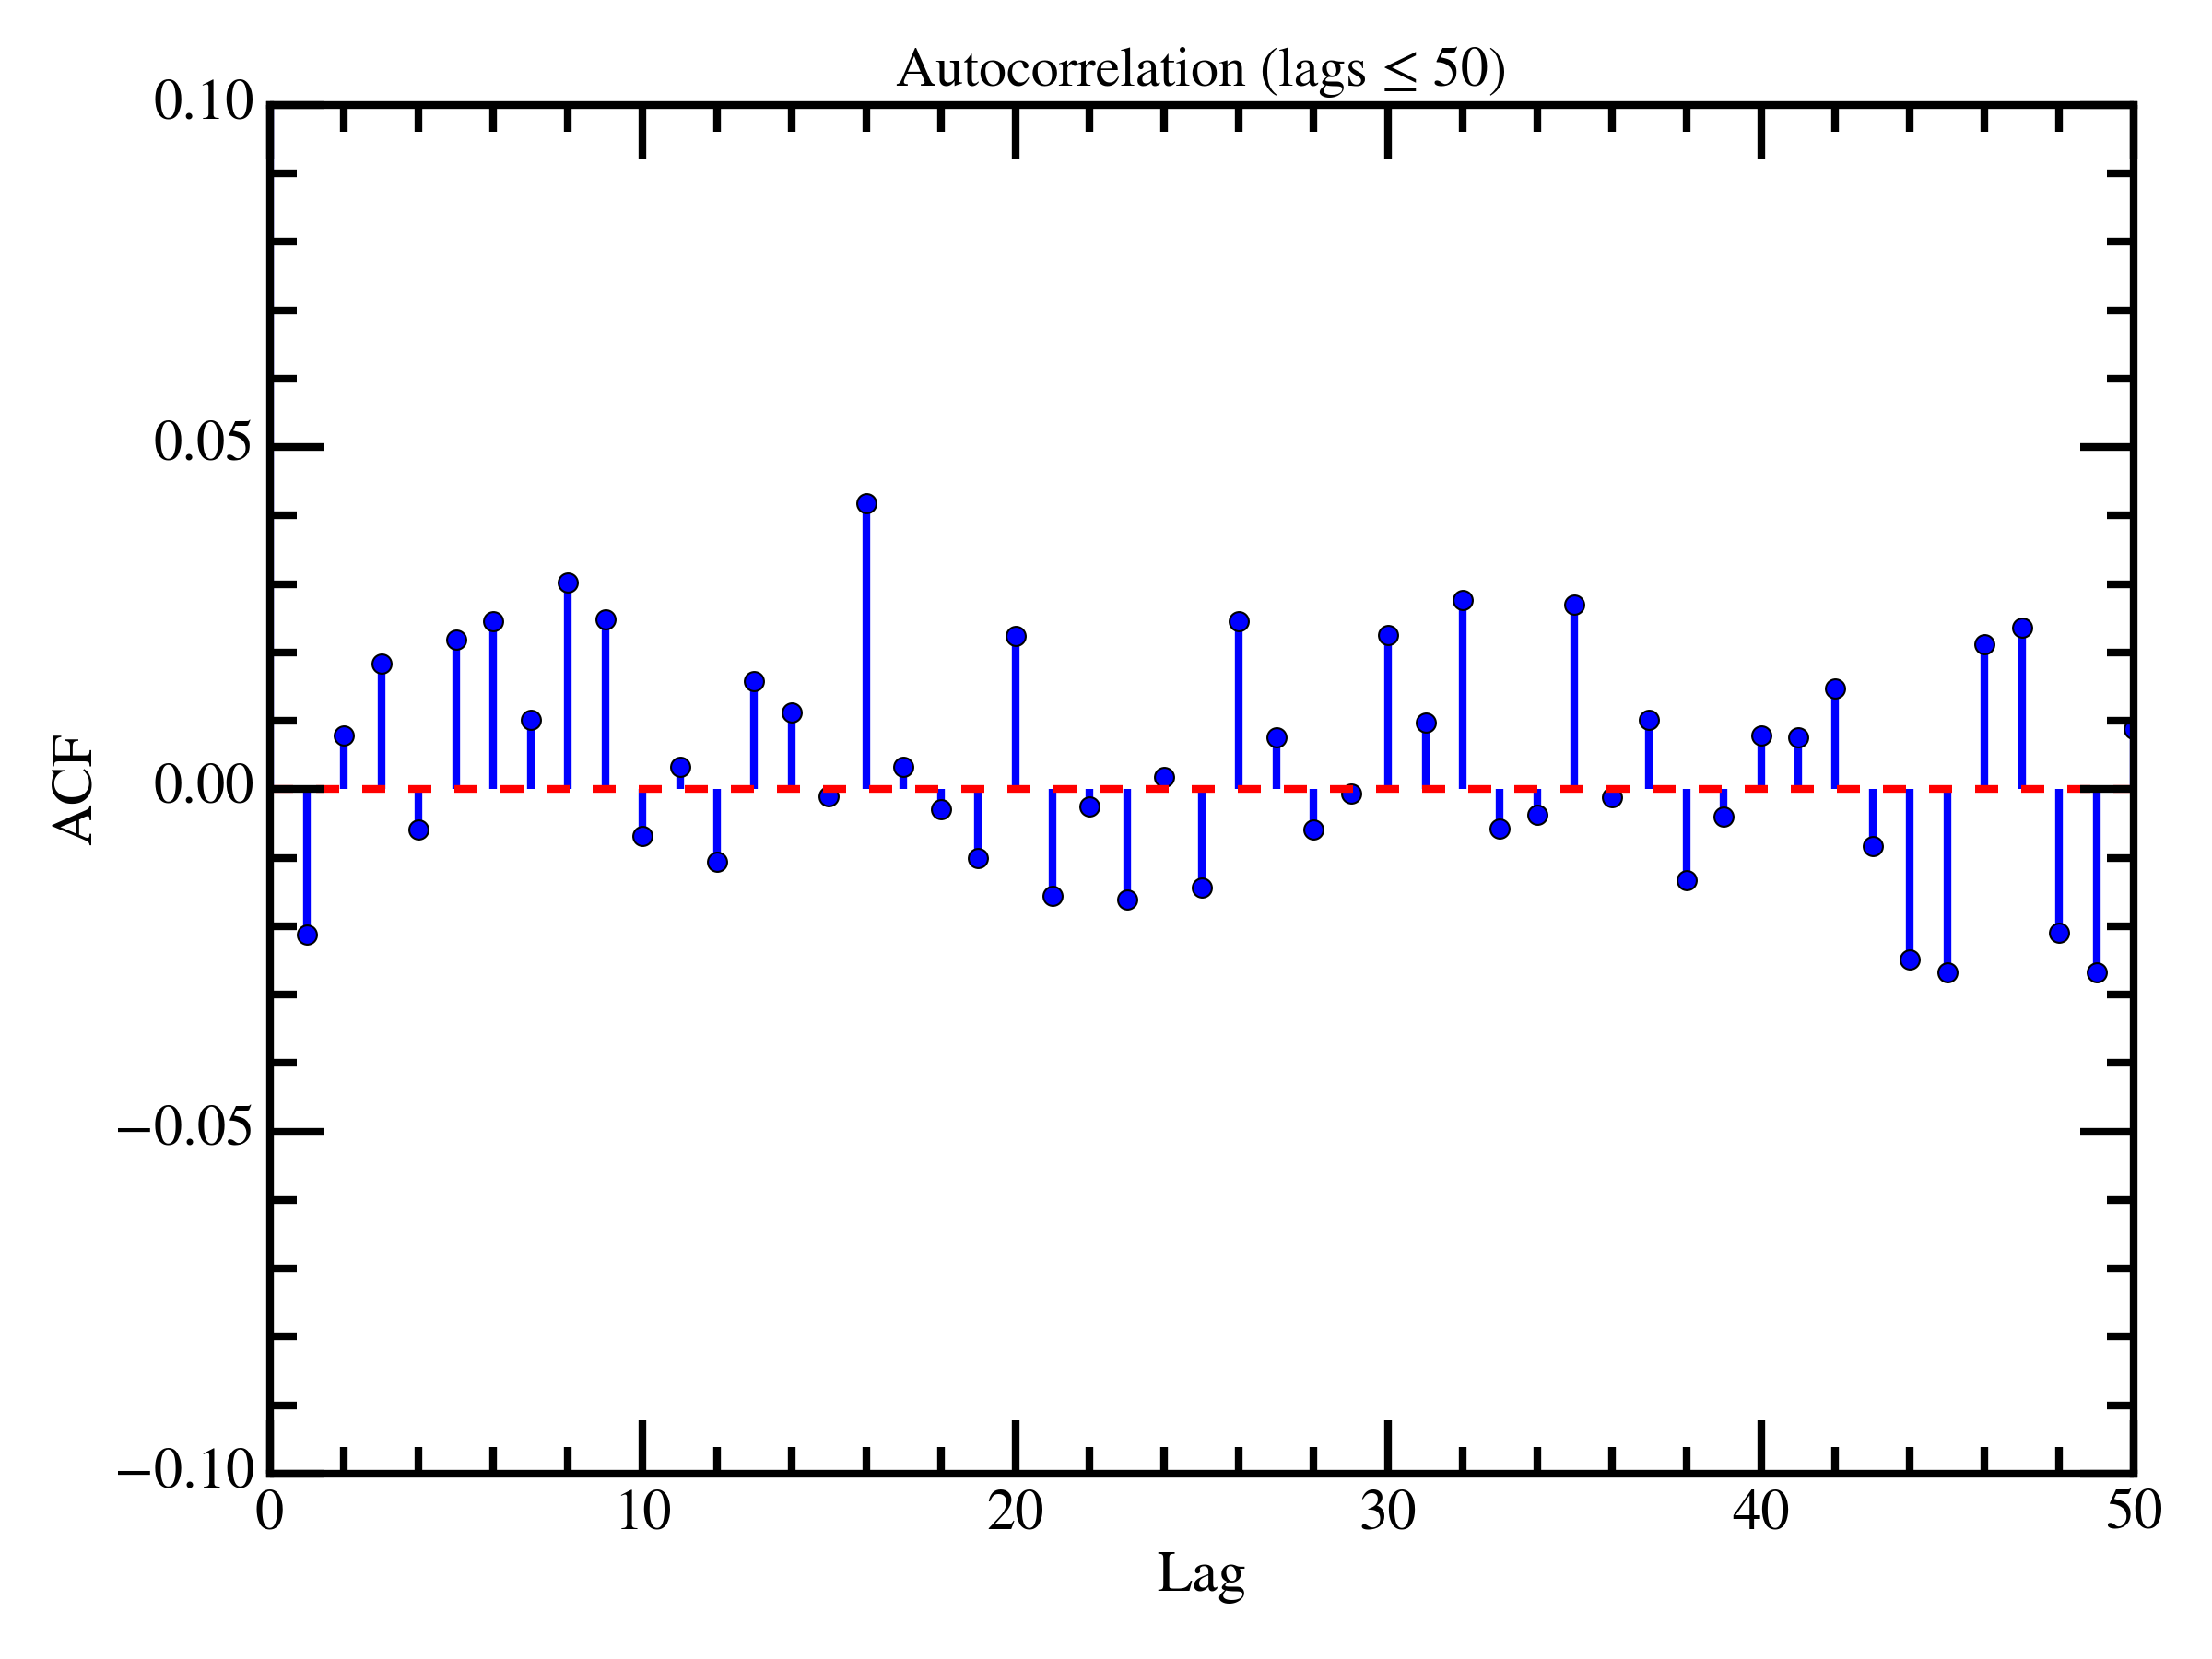
\includegraphics[width=0.45\textwidth]{figure/acf_bits.png}
\caption{Autocorrelation function of the binary sequence against the time lag. The plot shows that the autocorrelation function is close to zero, indicating that the data is random.}
\label{fig:autocorrelation}
\end{figure}

\subsection{Compression Ratio}

With \textsc{gzip}, we have a compression ratio of $1.11$. The reason for the compression ratio being greater than 1 is that the compression algorithm adds header information to the compressed data. 

\subsection{Entropy}

Next, we show the entropy of the binary sequence. The shannon entropy is $0.99982 \pm 0.00085$. The significance of the result compared to the expected value of 1 is $z=0.21$, which is not significant at the 5\% level. The entropy is close to 1, indicating that the data is random.

\subsection{Lempel-Ziv Complexity}

Next, we show the result of the Lempel-Ziv complexity test. With the length of the binary sequence $N=1636$, we expect $c(S) \sim \frac{n}{\log_2 n} = 258$. The observed Lempel-Ziv complexity is $c(S) = 258 \pm 1$. The significance of the result compared to the expected value of 258 is $z=0.00$, which is not significant at the 5\% level. 

\subsection{Angular Dependence Test}

Lastly, we show the dependence of the probability of getting a 1 in the sequence on the angle of the detectors in Fig. \ref{fig:angle_dependence}. We obtain the slope of the linear fit to be $-0.00072 \pm 0.00051$. The significance of the result compared to the expected value of 0 is $z=1.40$, which is not significant at the 5\% level. 

\begin{figure}
\centering
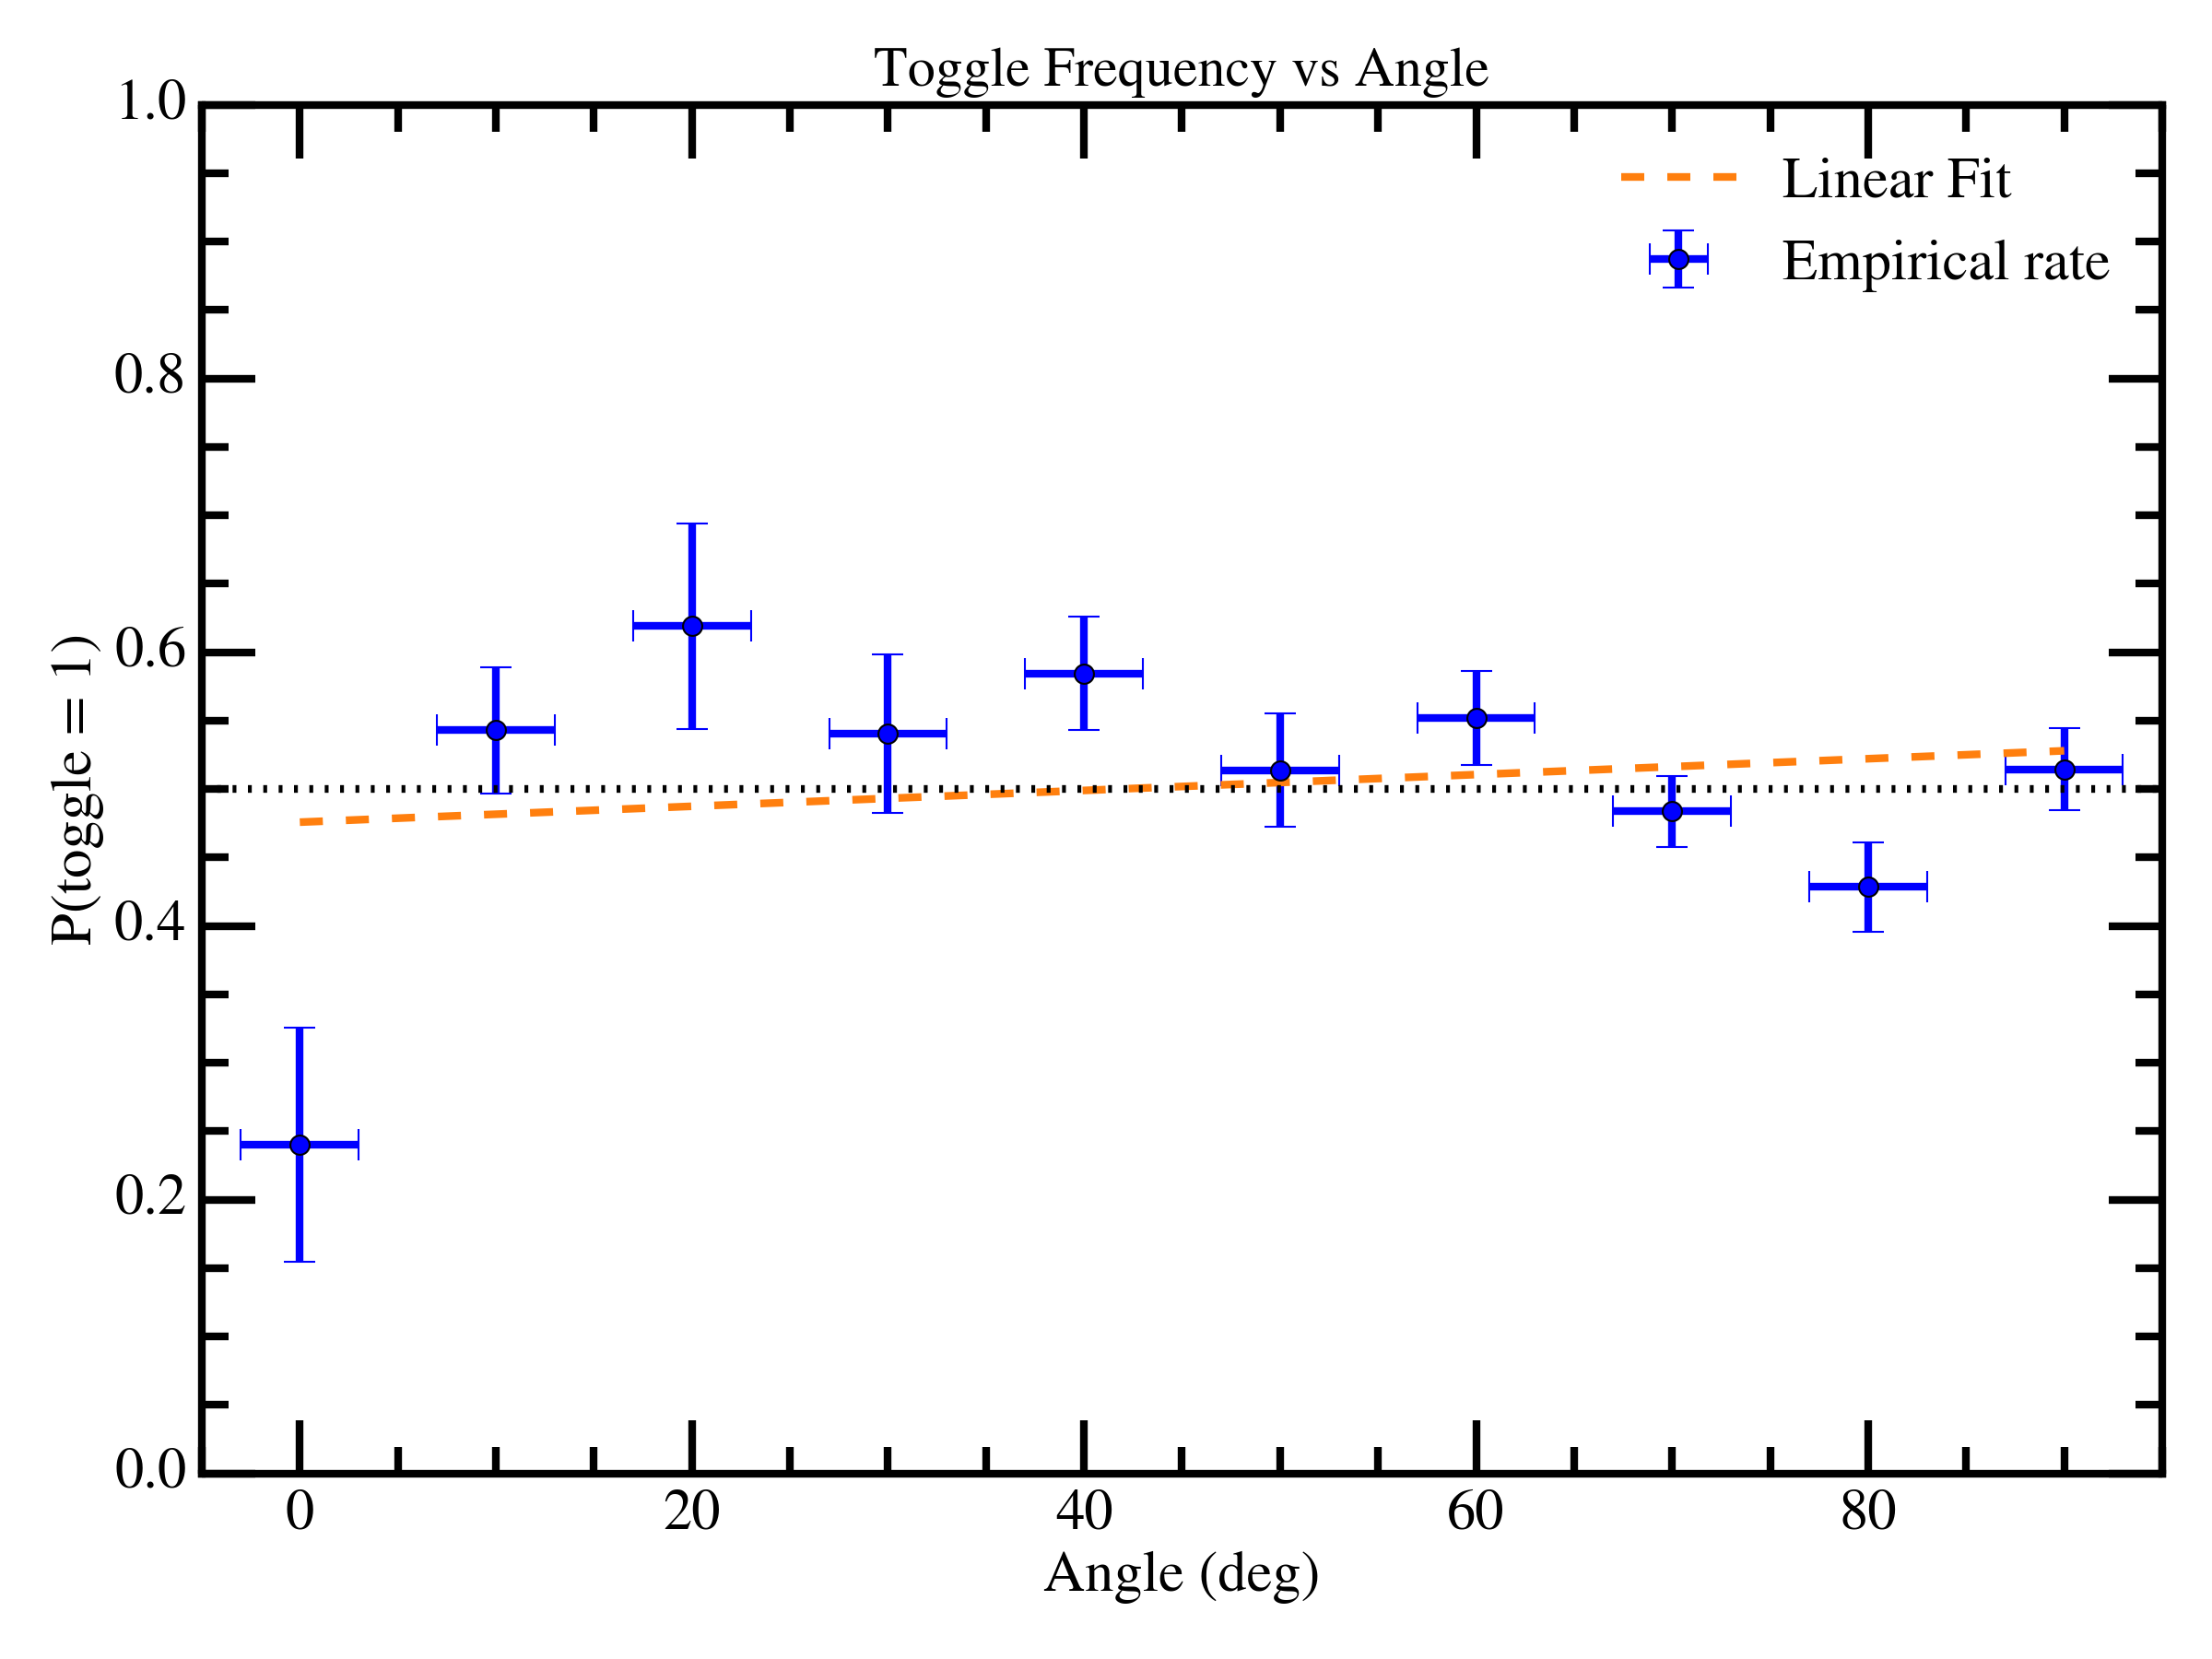
\includegraphics[width=0.45\textwidth]{figure/toggle_vs_angle.png}
\caption{Dependence of the probability of getting a 1 in the sequence on the angle of the detectors. The plot shows that the probability of getting a 1 in the sequence is roughly equal for all angles, indicating that the angle does not have a significant effect on the random nature of the data.}
\label{fig:angle_dependence}
\end{figure}

\subsection{Summary of Results}
The result of the analysis is summarized in Table \ref{tab:summary}. The table shows that all the tests indicate that the data is close to true randomness. The angular dependence test also shows that the angle does not have a significant effect on the random nature of the data. The combined level of signficance with Stouffer's method \cite {stouffer1949american} is $z=0.40$, which is not significant at the 5\% level. 
\begin{table*}
\centering
\begin{tabular}{|c|c|c|c|}
\hline
Test & Prediction & Result & Significance\\
\hline
Monobit Probability & 0.5 & $0.508 \pm 0.012$ & 0.64 \\
\hline
Autocorrelation Function & 0.0117 & $0.0172 \pm 0.0024$ & 1.06\\
\hline
Compression Ratio & 1 & $1.11$ & - \\
\hline
Shannon Entropy & 1 & $0.99982 \pm 0.00085$ & 0.21\\
\hline
Lempel-Ziv Complexity & $258$ & $258 \pm 1$ & 0 \\
\hline
Angular Dependence & 0 & $-0.00072 \pm 0.00051$ & 1.40\\
\hline
\end{tabular}
\caption{Summary of the results of the analysis. The table shows that all the tests indicate that the data is random. The angular dependence test also shows that the angle does not have a significant effect on the random nature of the data.}
\label{tab:summary}
\end{table*}

\section{Conclusion}
In conclusion, the analysis shows that the muon detection process is indeed random, with a deviation of $0.40\sigma$. The results of the statistical tests, including the autocorrelation function, sequence test, compression test, entropy test, and Lempel-Ziv complexity test, all indicate that the data is random. The analysis also shows that the angle of the detectors does not have a significant effect on the random nature of the data.

The results of the analysis are consistent with the expected behavior of a random process. The analysis also shows that the muon detection process is not affected by the angle of the detectors. 

The application of a true random number generator is important in many fields, including cryptography, simulations, and statistical analysis. The results of this analysis show that the muon detection process can indeed be used as a source of true random numbers. 



\begin{acknowledgments} The author gratefully acknowledges their lab partner V. Tran for their invaluable assistance. The author also thanks the 8.13 teaching team for their guidance in the lab. This work was supported by the MIT Department of Physics. 
\end{acknowledgments}

\bibliographystyle{abbrv}
\bibliography{ref}
\end{document}

